\subsection{Execute stage}
The combinatorial execute stage is where the execution of the instruction is done. The main components are the ALU and its control unit. In addition to the ALU control unit, which works as it did in the previous assignment \cite{multicycle}, the forwarding unit described in section \ref{section:forwarding_unit} has a control task in this stage. Figure~\ref{fig:stage_ex} shows the architecture of the stage.

\begin{figure}[h]
        \centering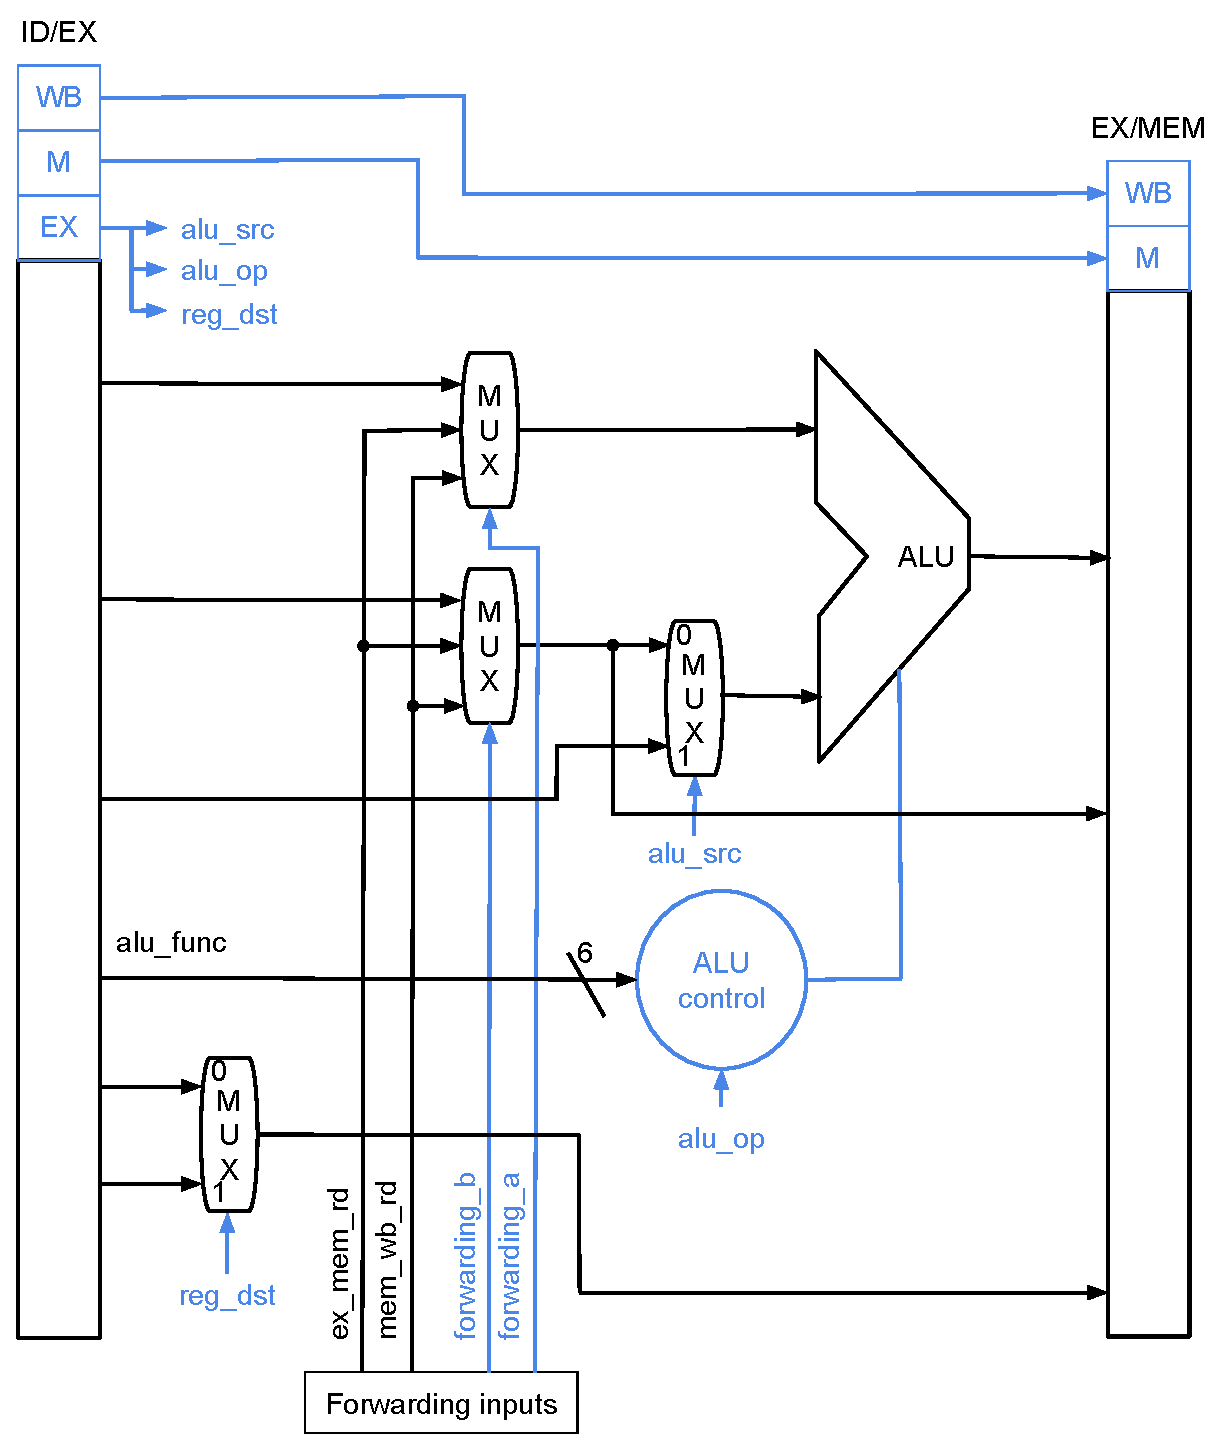
\includegraphics[scale=0.5]{figures/stage_ex}
        \caption{The stage\_ex architecture}
        \label{fig:stage_ex}
\end{figure}

The ALU inputs are controlled by three muxes. On each input there is one mux controlled by their respective forwarding control signals, that choose from what stage the input to the ALU is coming from. In addition there is a mux on the B input that, depending on the \emph{alu\_src} signal, chooses whether the forwarding controlled mux or the sign extended last 16 bit of the instruction should be input to the ALU. The forwarding muxes choose their input according to table~\ref{table:forwarding_results}. The execute stage also includes a mux that uses the \emph{reg\_dst} signal to choose which register should be written to in the memory stage.

\begin{table}[h]
    \begin{tabular}{ l | l | p{6.5cm} }
        Mux control & Source & Explanation \\
        \hline                        
        \emph{forwarding\_a} = 00 & ID/EX  & ALU operand A comes from the register file. \\
        \emph{forwarding\_a} = 10 & EX/MEM & ALU operand A is forwarded from the prior ALU result. \\
        \emph{forwarding\_a} = 01 & MEM/WB & ALU operand A is forwarded from data memory or an earlier ALU result.\\
        \hline
        \emph{forwarding\_b} = 00 & ID/EX  & ALU operand B comes from the register file. \\
        \emph{forwarding\_b} = 10 & EX/MEM & ALU operand B is forwarded from the prior ALU result. \\
        \emph{forwarding\_b} = 01 & MEM/WB & ALU operand B is forwarded from data memory or an earlier ALU result. \\
    \end{tabular}
    \caption{Forwarding mux source choosing}
    \label{table:forwarding_results}
\end{table}